%           - Header-           %
\documentclass[a4paper, 11pt, fleqn, notitlepage, egregdoesnotlikesansseriftitles]{scrartcl}
\usepackage[english, ngerman]{babel}                % Sprache: Deutsch
\usepackage[utf8]{inputenc}                         % Dateiformat
\usepackage[T1]{fontenc}                            % Schriftsatz

%       - wichtige Pakete -     %
\usepackage{kpfonts}                                % Schrift
\usepackage{geometry}                               % Struktur
\usepackage{hyperref}                               % klickbare links
\usepackage{amsmath, amssymb, mathtools}            % mathematische Formeln
\usepackage[headsepline]{scrlayer-scrpage}          % Kopf- und Fußzeilen konfigurieren

%       - nuetzliche Pakete -   %
%\usepackage{tabularx}                              % schöne tabellen
%\usepackage{booktabs}                              % Trennlinien in Tabellen
%\setlength{\columnsep}{0.7cm}                      % Spaltenabstand
%\usepackage{multicol}                              % mehrspaltiger Text
\usepackage{graphicx}                               % Grafiken
\usepackage[section]{placeins}
%\usepackage{tikz}                                  % Grafiken und Graphen
%\usepackage{diagbox}                               % Tabellen unterteilen
%\usepackage{bussproofs}                            % Logik und Kalkuele
%\usepackage{nicefrac}                              % schraege Brüche

% BibLateX
%\usepackage[backend=biber, authordate, eprint=false, url=false, block=ragged, bibencoding=inputenc]{biblatex-chicago}
%\usepackage{csquotes}
%\bibliography{quellen}                             % Quellen

%       - Eigene Befehle -      %
\newcommand{\emptyline}{\vspace{\baselineskip}}     % erzeugt leerzeile

%\newcommand{\N}{\mathbb{N}}
%\newcommand{\Z}{\mathbb{Z}}
%\newcommand{\R}{\mathbb{R}}
%\newcommand{\C}{\mathbb{C}}
%\newcommand{\Pf}{\mathbb{P}}

\newcommand{\aufgabe}{Block 6b}
\newcommand{\modul}{Rechnernetze und Verteilte Systeme}
\newcommand{\sem}{Wintersemester 18/19}
\newcommand{\autorA}{Daniel Wujecki}
\newcommand{\autorB}{Amro Hendawi}
\newcommand{\autorC}{Nils Hendrischke}
\newcommand{\autorD}{Leon Marius Moll}
\newcommand{\autoren}{Wujecki, Hendawi, Hendrischke, Moll}
\newcommand{\uni}{Technische Universität Berlin}
\newcommand{\datum}{\today}

%       - Einstellungen -       %
\title{\aufgabe}
\subtitle{\modul}
\author{\name}
\date{\datum}

%\setlength{\parindent}{0pt}                                        % einruecken verhindern
\pagestyle{scrheadings}
%\setcounter{secnumdepth}{0}                                        % keine Nummerierung von Überschriften
\geometry{left=25mm,right=20mm, top=27mm, bottom=25mm}              % bestimmte Seitenraender

\ihead{\aufgabe}
\chead{}
\ohead{\autoren}

\begin{document}

%         - Ttielseite -        %
%\maketitle
\thispagestyle{scrplain}

\noindent\Large
\textbf{\aufgabe} \hfill \textbf{\modul} \\
\normalsize
\autorA \hfill \uni \\
\autorB \hfill \sem \\
\autorC \hfill \datum \\
\autorD \hfill T18 G01 \\
\rule{\textwidth}{0.1mm}

%     - Inhaltsverzeichnis -    %
%\tableofcontents
%\newpage

%            - Text -           %

\section*{Ausgewählte Zeitserver}


{\setlength{\tabcolsep}{2pt}
\begin{tabular*}{\linewidth}{@{\extracolsep{\fill}}|l|c|c|l|l|@{}}
    \hline
    \textbf{Bezeichnung} & \textbf{Stratum} & \textbf{Uhr} & \textbf{Entfernung} & \textbf{Hostname} \\
    \hline
    tu-berlin & 1 & GPS & 0\,km & ntps1-0.eecsit.tu-berlin.de \\
    uni-erlangen & 1 & GPS & 366\,km & ntp0.rrze.uni-erlangen.de \\
    uni-paderborn & 1 & Funkuhr & 329\,km & time1.uni-paderborn.de \\
    uni-bielefeld & 2 & & 336\,km & stratum2-4.NTP.TechFak.Uni-Bielefeld.DE \\
    mazzanet-australia & 2 & & 15.900\,km & ntp.mazzanet.net.au \\
    \hline
\end{tabular*}}

\emptyline
Für jeden Server wurden 100 aufeinander folgende Messungen mit 6 Sekunden Abstand gemacht.
Bei jeder Messung wurde dabei als Client ein NTP-Paket der Version 4 verschickt und die Antwort vom Server empfangen. Die Messungen der verschiedenen Server wurden sequentiell ausgeführt, sind also voneinander zeitlich unabhängig. Die Daten wurden in einer CSV--Datei gesammelt und dann mittels der \verb+python3+ Bibliothek \verb+matplotlib+ graphisch veranschaulicht. Die Abbildungen mit der meisten Aussagekraft haben wir ausgewählt und in diesem Dokument dargestellt.

\newpage
\section*{Plots nach Offset, Delay und Root Dispersion}
\vspace{-\baselineskip}

\begin{center}
    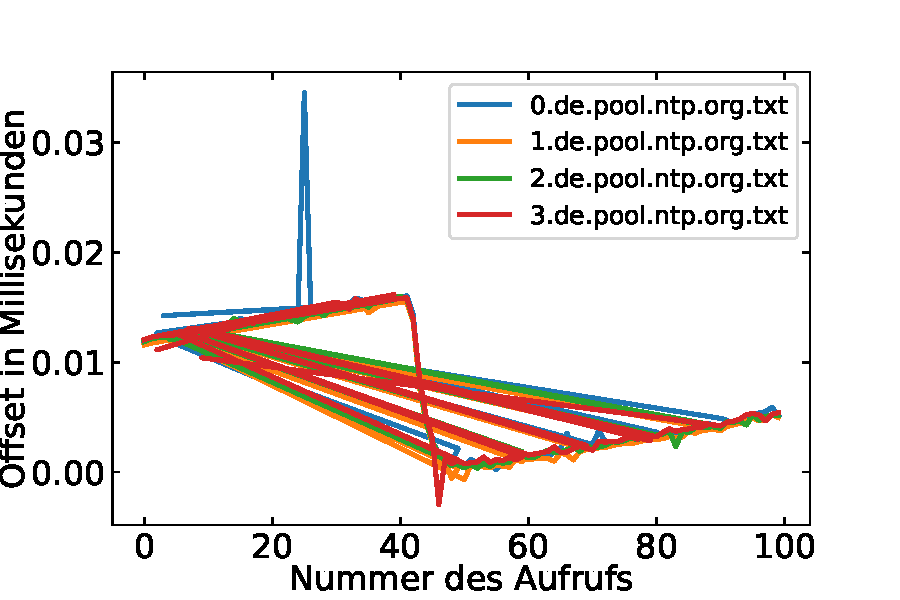
\includegraphics[width=\textwidth]{together/Offset_all.pdf}
    \captionof{figure}{Offset von allen Zeitservern}
    \label{fig:offset}
\end{center}

Bis auf den australischen Server verhalten sich alle Server annähernd gleichmäßig. Das bedeutet, dass die Uhren von Client und Server ähnlich schnell laufen. Die Ausreißer, zu erkennen als große Ausschläge der Graphen, sind damit zu erklären, dass die Pakete in einigen Fällen anders geroutet wurden und somit länger brauchten. Der australische Server ist sehr weit entfernt und hat in der Summe somit ein höhreres Offset. Aufgrund der großen Entfernung gibt es wesentlich mehr Knotenpunkte über die das Paket geleitet werden kann und somit viele verschiedene Routen mit unterschiedlichen Offsets.

\begin{center}
    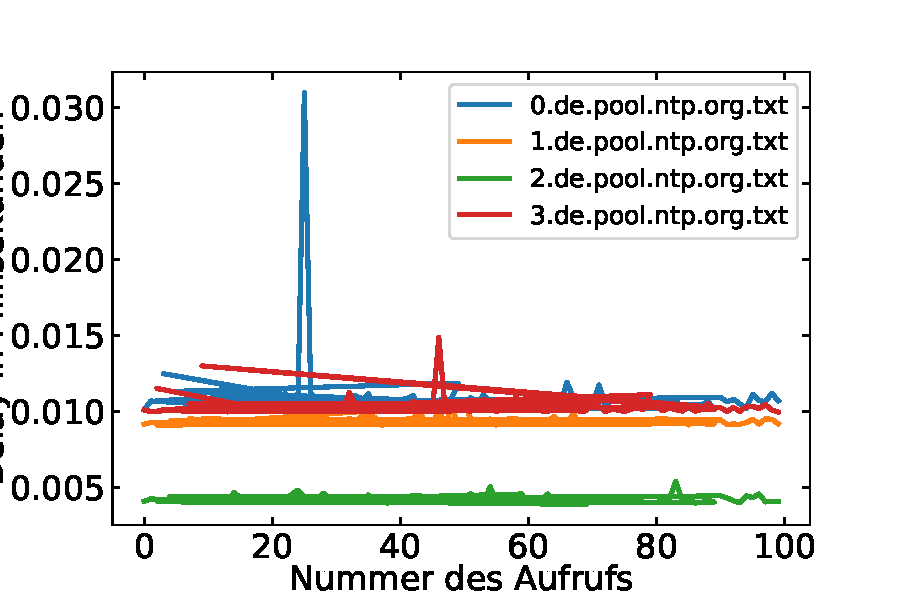
\includegraphics[width=\textwidth]{together/Delay_all.pdf}
    \captionof{figure}{Delay von allen Zeitservern}
    \label{fig:delay}
\end{center}

Das Delay ist dem Standort der Server entsprechend. Somit ergibt sich ein hohes Delay für Australien, den mit Abstand am weitesten entfernten Server. Die Delays der deutschen Server fallen entsprechend gering aus. Besonders klein ist das Delay des Servers der TU-Berlin, da zu diesem Server praktisch keine geographische Entfernung vorhanden ist. Die vereinzelten Ausreißer aller Server lassen sich wieder mit dem unterschiedlichen Routen der Pakete erklären.

\begin{center}
    \includegraphics[width=\textwidth]{together/root_dispersion.pdf}
    \captionof{figure}{Root Dispersion von zwei Zeitservern}
    \label{fig:disp}
\end{center}

Die Root Dispersion gibt die Abweichung der Uhr des Servers zu seiner Zeitquelle an. Am Graphen kann man ablesen, dass die Uhr des Zeitservers auch nie exakt läuft, sondern immer ein bisschen langsamer oder schneller im Vergleich zu seiner Zeitquelle. In regelmäßigen Zeitabständen synchronisiert sich der Server wieder mit seiner Zeitquelle. Zu diesen Zeitpunkten fällt die Root Dispersion besonders klein aus.

Auffällig ist es, dass die Messwerte im Mikrosekundenbereich immer wieder stark ausschlagen, wohingegen die Messwerte von Offset und Delay sich im Millisekundenbereich befinden und eher kontinuierlich verlaufen. Das starke Ausschlagen ist damit zu begründen, dass wir alle 6 Sekunden Messungen vorgenommen haben. Dieses Interval ist offenbar so groß, dass man die Entwicklung der Root Dispersion nicht genau nachhvollziehen kann und entweder eine Verhältnismäßig kleine oder große Root Dispersion als Messergebnis bekommt.

Damit die Abbildung möglichst übersichtlich bleibt, haben wir nur die Root Dispersion von zwei Servern dargestellt.

\section*{Plots nach Zeitservern}

\begin{center}
    \includegraphics[width=\textwidth]{server/uni-bielefeld.pdf}
    \captionof{figure}{Alle Daten Uni-Bielefeld}
    \label{fig:bielefeld}
\end{center}

Das Offset fällt bei ungefähr 70 Anfragen stark ab, während das Delay stabil bleibt. Das lässt darauf schließen, dass sich entweder der Computer, auf dem die Messungen laufen, oder der Server mit einer Zeitquelle synchronisiert hat und die Differenzen zwischen beiden Uhren damit kleiner ausfällt.

\begin{center}
    \includegraphics[width=\textwidth]{server/uni-paderborn.pdf}
    \captionof{figure}{Alle Daten Uni-Paderborn}
    \label{fig:paderborn}
\end{center}

Bei dieser Abbildung kann man sehr gut einen Zusammenhang zwischen Delay und Offest erkennen. Wenn das Delay sehr groß ist, also die Übertragung von Anfrage und Antwort sehr lange dauert, schlägt auch das Offset entsprechend aus und wir damit ungenau und nicht zuverlässig. Aus diesem Grund wählt man am liebsten das Offset eines Paketes, das ein kleines Delay hat.

\begin{center}
    \includegraphics[width=\textwidth]{server/mazzanet-australia.pdf}
    \captionof{figure}{Alle Daten mazzanet-australia}
    \label{fig:mazzanet}
\end{center}

\section*{Plots nach Messungen}

\begin{center}
    \includegraphics[width=\textwidth]{diff/uni-bielefeld_compare_Offset.pdf}
    \captionof{figure}{Offset zweier Messung Uni-Bielefeld}
    \label{fig:diff:bielefeld:offset}
\end{center}

Während der einen Messung fand offenbar eine Synchronisierung statt, währen das Offset bei der anderen Messung, sowie die beiden zugehörigen Delays, weitestgehend stabil bleiben.

\begin{center}
    \includegraphics[width=\textwidth]{diff/uni-bielefeld_compare_Delay.pdf}
    \captionof{figure}{Delay zweier Messung Uni-Bielefeld}
    \label{fig:diff:bielefeld:delay}
\end{center}

\begin{center}
    \includegraphics[width=\textwidth]{diff/uni-paderborn_compare_Offset.pdf}
    \captionof{figure}{Offset zweier Messung Uni-Paderborn}
    \label{fig:diff:paderborn:offst}
\end{center}

Die Offsets zweier verschiedener Messungen fallen gleichmäßig, aber sehr unterschiedlich in ihrem Wertebereich aus. Man kann Schlussfolgern, dass die Uhr des Computers, auf dem die Messungen vorgenommen wurden, oder des Servers unsynchronisiert waren und während der Messung nicht synchronisiert wurden. Die Vorraussetzung für diese Schlussfolgerung ist, dass die beiden Delays ungefähr gleich groß bleiben. Das kann man bei der folgenden Abbildung jedoch gut nachvollziehen.

\begin{center}
    \includegraphics[width=\textwidth]{diff/uni-paderborn_compare_Delay.pdf}
    \captionof{figure}{Delay zweier Messung Uni-Paderborn}
    \label{fig:diff:paderborn:delay}
\end{center}

%     - Quellenverzeichnis -    %
%\newpage
%\printbibliography

\end{document}
